\documentclass[oneside,14pt]{extarticle}
\usepackage[utf8]{inputenc}
\usepackage[english,ukrainian]{babel}
\usepackage{amssymb,amsfonts,amsmath,amsthm,mathtext,textcomp}
%\usepackage{fontspec}
% \setmainfont[Mapping=tex-text]{Times New Roman}
\usepackage[includehead, headsep=0pt, footskip=0pt, top=2cm, bottom=2cm, left=2cm, right=1cm]{geometry}
\usepackage{indentfirst}
\usepackage[onehalfspacing]{setspace}
\usepackage[headings]{fancyhdr}
\usepackage{etoolbox}
\usepackage{flafter}
\usepackage{listings}
\usepackage{graphicx}
\usepackage{float}
\usepackage[labelsep=period]{caption}
\lstset{
	breaklines=false
}
\usepackage{array}
\fancyhf{}
\renewcommand{\headrulewidth}{0pt}
\pagestyle{fancy}
\fancyfoot[R]{\thepage}
\lstset{breaklines=true,}
\graphicspath{ {./pictures} }

\lstset{
	language=c,
	tabsize=4,
	keepspaces,
	showstringspaces=false,
}
\graphicspath{ {./pictures} }
\setlength{\parindent}{4em}
\setlength\tabcolsep{5px}

\newcommand\subject{Комп'ютерна графіка}
\newcommand\lecturer{доцент кафедри ПЗ \\ Левус Є. В.}
\newcommand\teacher{доцент кафедри ПЗ \\ Левус Є. В.}
\newcommand\mygroup{ПЗ-32}
\newcommand\lab{1-4}
\newcommand\theme{}
\newcommand\purpose{}

\begin{document}
\begin{normalsize}
	\begin{titlepage}
		\thispagestyle{empty}
		\begin{center}
			\textbf{МІНІСТЕРСТВО ОСВІТИ І НАУКИ УКРАЇНИ\\
				НАЦІОНАЛЬНИЙ УНІВЕРСИТЕТ "ЛЬВІВСЬКА ПОЛІТЕХНІКА"}
		\end{center}
		\begin{flushright}
			\textbf{ІКНІ}\\
			Кафедра \textbf{ПЗ}
		\end{flushright}
		\vspace{70pt}
		\begin{center}
			\textbf{ЗВІТ}\\
			про виконання лабораторних робіт № \lab\\
			\textbf{з дисципліни}: <<\subject>>\\
			\textbf{варіант}:  індивідуальний №2
		\end{center}
		\vspace{50pt}
		\begin{flushright}
			
			\textbf{Лектор}:\\
			\lecturer\\
			\vspace{10pt}
			\textbf{Виконав}:\\
			
			студент групи \mygroup\\
			Коваленко Д.М.\\
			\vspace{10pt}
			\textbf{Прийняла}:\\
			
			\teacher\\
			
			\vspace{28pt}
			«\rule{1cm}{0.15mm}» \rule{1.5cm}{0.15mm} 2023 р.\\
			$\sum$ = \rule{1cm}{0.15mm}……………\\
			
		\end{flushright}
		\vspace{\fill}
		\begin{center}
			\textbf{Львів — 2023}
		\end{center}
	\end{titlepage}

	\tableofcontents
	\pagebreak
	
	\section{Завдання}
	\subsection{Індивідуальний варіант}
	\begin{enumerate}
		\item[1)] Побудувати фрактальні зображення: \begin{enumerate}
			\item[1.1)] Фрактал Мандельброта $f(z)=z\cdot z+c$. Можливість згенерувати різні
			зображення, а саме для: \begin{enumerate}
				\item[-] різних кольорових схем,
				\item[-] різного масштабування.
			\end{enumerate}
			\item[1.2)] Броунівський рух.
		\end{enumerate}
		\item[2)] Колірні моделі: RGB і HSV. Змінити насиченість по зеленому кольору.
		\item[3)] Реалізувати рух для паралелограма, введеного за його вершинами, на основі
		повороту за годинниковою стрілкою відносно вибраної вершини з одночасним його
		зменшення у А разів.
	\end{enumerate}

	\begin{figure}[H]
		\centering
		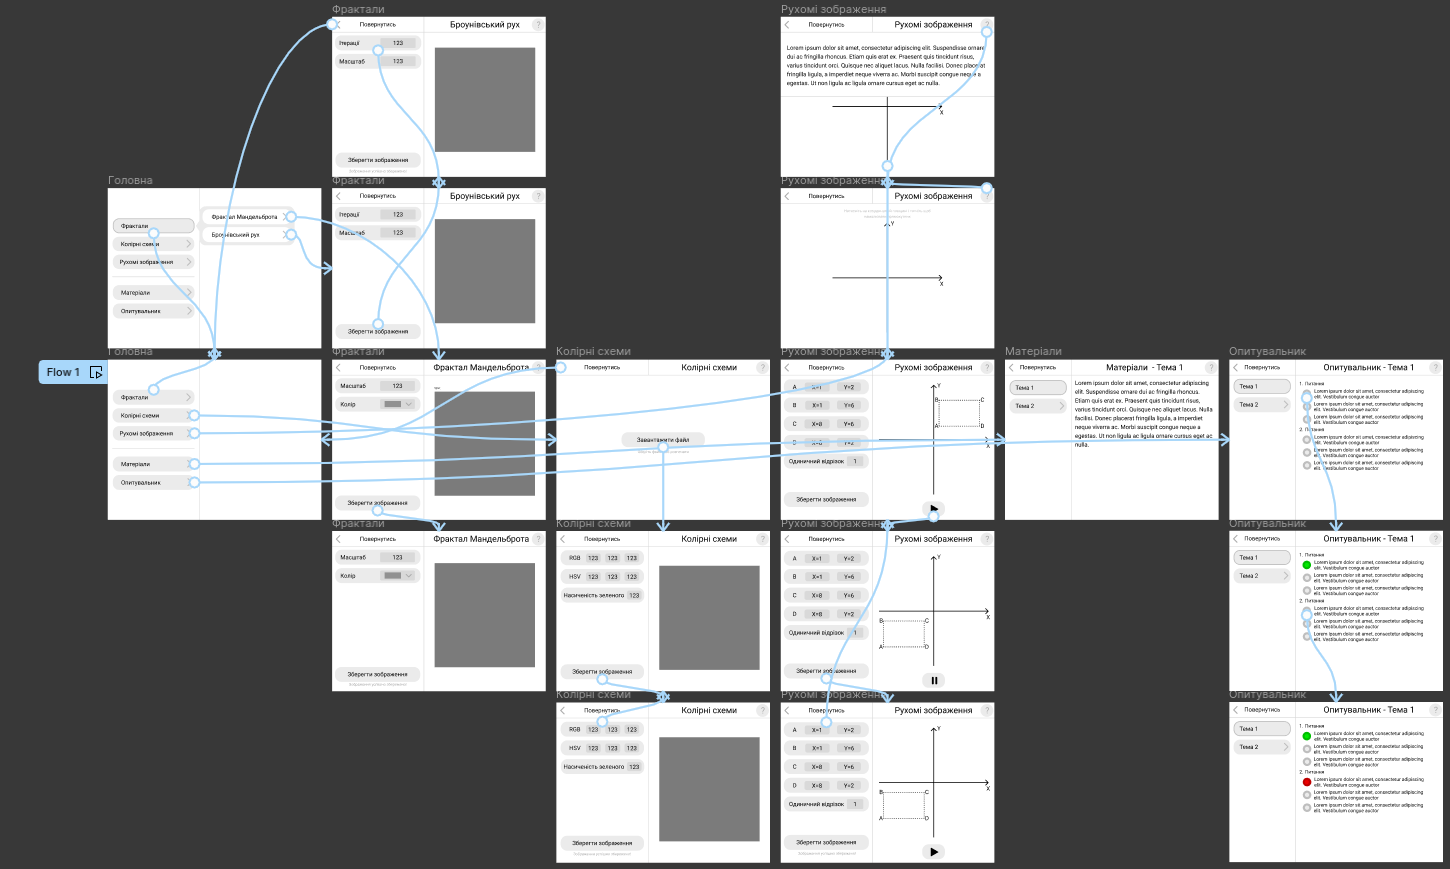
\includegraphics[scale=0.45]{wireflow}
		\caption{Wireflow}
	\end{figure}

	\section{Теоретичні відомості}
	\subsection{Опис функцій програми}
	\subsection{Алгоритми фракталів}
	\subsection{Анотація кольорових моделей}
	\subsection{Оптимальний матричний вираз афінних перетворень}
	\subsection{Реалізація графічного режиму}
	
	\section{Результати}

	\section{Висновки}
	   
	 \section{Список використаних інформаційних джерел}
\end{normalsize}
\end{document}
